% Options for packages loaded elsewhere
\PassOptionsToPackage{unicode}{hyperref}
\PassOptionsToPackage{hyphens}{url}
\PassOptionsToPackage{dvipsnames,svgnames,x11names}{xcolor}
%
\documentclass[
  letterpaper,
  DIV=11,
  numbers=noendperiod]{scrartcl}

\usepackage{amsmath,amssymb}
\usepackage{iftex}
\ifPDFTeX
  \usepackage[T1]{fontenc}
  \usepackage[utf8]{inputenc}
  \usepackage{textcomp} % provide euro and other symbols
\else % if luatex or xetex
  \usepackage{unicode-math}
  \defaultfontfeatures{Scale=MatchLowercase}
  \defaultfontfeatures[\rmfamily]{Ligatures=TeX,Scale=1}
\fi
\usepackage{lmodern}
\ifPDFTeX\else  
    % xetex/luatex font selection
\fi
% Use upquote if available, for straight quotes in verbatim environments
\IfFileExists{upquote.sty}{\usepackage{upquote}}{}
\IfFileExists{microtype.sty}{% use microtype if available
  \usepackage[]{microtype}
  \UseMicrotypeSet[protrusion]{basicmath} % disable protrusion for tt fonts
}{}
\makeatletter
\@ifundefined{KOMAClassName}{% if non-KOMA class
  \IfFileExists{parskip.sty}{%
    \usepackage{parskip}
  }{% else
    \setlength{\parindent}{0pt}
    \setlength{\parskip}{6pt plus 2pt minus 1pt}}
}{% if KOMA class
  \KOMAoptions{parskip=half}}
\makeatother
\usepackage{xcolor}
\setlength{\emergencystretch}{3em} % prevent overfull lines
\setcounter{secnumdepth}{-\maxdimen} % remove section numbering
% Make \paragraph and \subparagraph free-standing
\ifx\paragraph\undefined\else
  \let\oldparagraph\paragraph
  \renewcommand{\paragraph}[1]{\oldparagraph{#1}\mbox{}}
\fi
\ifx\subparagraph\undefined\else
  \let\oldsubparagraph\subparagraph
  \renewcommand{\subparagraph}[1]{\oldsubparagraph{#1}\mbox{}}
\fi


\providecommand{\tightlist}{%
  \setlength{\itemsep}{0pt}\setlength{\parskip}{0pt}}\usepackage{longtable,booktabs,array}
\usepackage{calc} % for calculating minipage widths
% Correct order of tables after \paragraph or \subparagraph
\usepackage{etoolbox}
\makeatletter
\patchcmd\longtable{\par}{\if@noskipsec\mbox{}\fi\par}{}{}
\makeatother
% Allow footnotes in longtable head/foot
\IfFileExists{footnotehyper.sty}{\usepackage{footnotehyper}}{\usepackage{footnote}}
\makesavenoteenv{longtable}
\usepackage{graphicx}
\makeatletter
\def\maxwidth{\ifdim\Gin@nat@width>\linewidth\linewidth\else\Gin@nat@width\fi}
\def\maxheight{\ifdim\Gin@nat@height>\textheight\textheight\else\Gin@nat@height\fi}
\makeatother
% Scale images if necessary, so that they will not overflow the page
% margins by default, and it is still possible to overwrite the defaults
% using explicit options in \includegraphics[width, height, ...]{}
\setkeys{Gin}{width=\maxwidth,height=\maxheight,keepaspectratio}
% Set default figure placement to htbp
\makeatletter
\def\fps@figure{htbp}
\makeatother
% definitions for citeproc citations
\NewDocumentCommand\citeproctext{}{}
\NewDocumentCommand\citeproc{mm}{%
  \begingroup\def\citeproctext{#2}\cite{#1}\endgroup}
\makeatletter
 % allow citations to break across lines
 \let\@cite@ofmt\@firstofone
 % avoid brackets around text for \cite:
 \def\@biblabel#1{}
 \def\@cite#1#2{{#1\if@tempswa , #2\fi}}
\makeatother
\newlength{\cslhangindent}
\setlength{\cslhangindent}{1.5em}
\newlength{\csllabelwidth}
\setlength{\csllabelwidth}{3em}
\newenvironment{CSLReferences}[2] % #1 hanging-indent, #2 entry-spacing
 {\begin{list}{}{%
  \setlength{\itemindent}{0pt}
  \setlength{\leftmargin}{0pt}
  \setlength{\parsep}{0pt}
  % turn on hanging indent if param 1 is 1
  \ifodd #1
   \setlength{\leftmargin}{\cslhangindent}
   \setlength{\itemindent}{-1\cslhangindent}
  \fi
  % set entry spacing
  \setlength{\itemsep}{#2\baselineskip}}}
 {\end{list}}
\usepackage{calc}
\newcommand{\CSLBlock}[1]{\hfill\break\parbox[t]{\linewidth}{\strut\ignorespaces#1\strut}}
\newcommand{\CSLLeftMargin}[1]{\parbox[t]{\csllabelwidth}{\strut#1\strut}}
\newcommand{\CSLRightInline}[1]{\parbox[t]{\linewidth - \csllabelwidth}{\strut#1\strut}}
\newcommand{\CSLIndent}[1]{\hspace{\cslhangindent}#1}

\KOMAoption{captions}{tableheading}
\makeatletter
\@ifpackageloaded{caption}{}{\usepackage{caption}}
\AtBeginDocument{%
\ifdefined\contentsname
  \renewcommand*\contentsname{Table of contents}
\else
  \newcommand\contentsname{Table of contents}
\fi
\ifdefined\listfigurename
  \renewcommand*\listfigurename{List of Figures}
\else
  \newcommand\listfigurename{List of Figures}
\fi
\ifdefined\listtablename
  \renewcommand*\listtablename{List of Tables}
\else
  \newcommand\listtablename{List of Tables}
\fi
\ifdefined\figurename
  \renewcommand*\figurename{Figure}
\else
  \newcommand\figurename{Figure}
\fi
\ifdefined\tablename
  \renewcommand*\tablename{Table}
\else
  \newcommand\tablename{Table}
\fi
}
\@ifpackageloaded{float}{}{\usepackage{float}}
\floatstyle{ruled}
\@ifundefined{c@chapter}{\newfloat{codelisting}{h}{lop}}{\newfloat{codelisting}{h}{lop}[chapter]}
\floatname{codelisting}{Listing}
\newcommand*\listoflistings{\listof{codelisting}{List of Listings}}
\makeatother
\makeatletter
\makeatother
\makeatletter
\@ifpackageloaded{caption}{}{\usepackage{caption}}
\@ifpackageloaded{subcaption}{}{\usepackage{subcaption}}
\makeatother
\ifLuaTeX
  \usepackage{selnolig}  % disable illegal ligatures
\fi
\usepackage{bookmark}

\IfFileExists{xurl.sty}{\usepackage{xurl}}{} % add URL line breaks if available
\urlstyle{same} % disable monospaced font for URLs
\hypersetup{
  pdftitle={Missoula Aquifer Sustainability Study},
  pdfauthor={Adaptive Hydrology},
  colorlinks=true,
  linkcolor={blue},
  filecolor={Maroon},
  citecolor={Blue},
  urlcolor={Blue},
  pdfcreator={LaTeX via pandoc}}

\title{Missoula Aquifer Sustainability Study}
\author{Adaptive Hydrology}
\date{2024-08-27}

\begin{document}
\maketitle

\subsection{Executive Summary}\label{executive-summary}

\begin{enumerate}
\def\labelenumi{\arabic{enumi}.}
\tightlist
\item
  The Missoula Aquifer is one of only 64 designated sole source aquifers
  in the United States. As such, it supplies over 75,000 residents, plus
  businesses, with potable groundwater. Its hydrogeology (e.g.~high
  transmissivity rates) and geography (e.g.~downstream location within
  the Clark Fork and Bitterroot watersheds) have created a resource that
  has been relatively resilient and predictable over the past
  23-years.\\
\item
  Due to the unconfined nature of the aquifer and the high
  transmissivity rates of the geological substrate, the upstream inflows
  (recharge) and downstream outflows (discharge), are largely controlled
  by the magnitude and timing of the Clark Fork River. In fact, the
  Clark Fork River provides over 80\% of the annual aquifer recharge.
  Thus, it is fair to say that any long-term changes in the streamflow
  will likely have far reaching impacts to the sustainability of the
  aquifer.\\
\item
  Over the past 23-years, population has increased from approximately
  57,000 to 78,000 people, roughly translating to an increase in water
  use of almost 40\%. According to the Montana Ground Water Information
  Center (GWIC) there are currently over 3,500 wells listed in the
  Missoula area. Of those wells, 247 are labeled as public water, which
  includes the City of Missoula's water supply. Population is expected
  to continue to increase over the next few decades, and assuming water
  use per resident remains consistent, more withdrawals will be
  necessary to keep up with this growing demand.\\
\item
  Climate change is expected to create additional stressors. Increases
  in temperature and shifts in snowpack runoff may reduce water
  availability during critical periods of high demand. In addition, when
  drought does occur, the magnitude and duration is expected to be worse
  than historical conditions.
\item
  In spite of the historical changes in population and temperature, the
  aquifer has been remarkably resilient over the past 23-years. All 16
  of the wells used in this analysis have shown increasing average
  trends over the study period. Additionally, minimum and maximum annual
  depths have been increasing over this same time period.\\
\item
  These increasing trends are almost entirely driven by the increasing
  annual and seasonal flows of the Clark Fork River. Trends in spring
  runoff have increased the most during the study period (113
  cfs/season) and have likely led to increases in recharge during the
  summer, when demand is highest. This has created an opportunitistic
  situation where the timing of maximum supply and demand are perfectly
  aligned. Unfortunately, there is large uncertainty as to whether this
  trend and timing in streamflow/recharge will continue into the
  future.\\
\item
  When removing the impact of the increasing trend in the Clark Fork
  River, the groundwater signal is driven by pumping rates (i.e.~overall
  water demand). Increasing demand leads towards statistically
  significant decreasing (i.e.~unsustainable) trends in groundwater. In
  addition, over the most recent 10-years, when the Clark Fork River
  flows have not increased, there are statistically significant
  decreasing trends in groundwater, which appear to be correlated with
  increasing withdrawals to match demand.
\item
  Aquifer withdrawals are highly correlated with temperature. As
  temperature increases, pumping rates have historically increased
  exponentially. In fact, temperature alone explains almost 95\% of the
  variation in pumping rates. This suggests that groundwater levels have
  been and will continue to be sensitive to climate change due to
  increases in demand to go along with potential decreases in recharge.
\item
  Further analysis using physics or machine/deep learning is recommended
  in order to better understand tipping points created from shifts in
  discharge timing and magnitude, as well as increases in population.
  This analysis might also allow for improved management decisions based
  on real-time and near-time estimates of groundwater sustainability.
\item
  Given that the aquifer does appear to be sensitive to climate change
  and withdrawals, it is imperative to be thinking now, while the
  aquifer is still resilient and plentiful, about ways to maintain a
  clean and copious groundwater resource for the City of Missoula and
  beyond.
\end{enumerate}

\subsection{Introduction}\label{introduction}

The Missoula Aquifer is one of only 64 designated sole source aquifers
in the United States.\footnote{https://www.epa.gov/dwssa} As such, it
supplies over 75,000 residents, plus businesses, with potable
groundwater. Historically, the aquifer has shown incredible resilience
to drought and increases in population within the Missoula valley area.
There have been no long-term signs of depletion in any of the 27
monitoring wells within the aquifer. This is likely due to the very high
transmissivity rates, location within the Clark Fork and Bitterroot
watersheds, reasonable historical growth rates of the surrounding
population, and only mild changes in historical climate (Whitlock et al.
2017).

Due to the unconfined nature of the aquifer and the high transmissivity
rates of the substrate, the upstream inflows, and downstream outflows,
of the aquifer are largely driven by the Clark Fork River (Tallman 2005;
Miller 1991). In fact, according to previous studies, the Clark Fork
River provides over 80\% of the annual aquifer recharge
(Table~\ref{tbl-miller}). Thus, it is fair to say that any long-term
changes in streamflow will likely have far reaching impacts to the
recharge and overall sustainability of the aquifer.

\begin{longtable}[]{@{}lll@{}}

\caption{\label{tbl-miller}Missoula aquifer source of average annual
inflow according to Miller (1991).}

\tabularnewline

\caption{}\label{T_312d3}\tabularnewline
\toprule\noalign{}
Source & Inflow (af/yr) & Percent of Total \\
\midrule\noalign{}
\endfirsthead
\toprule\noalign{}
Source & Inflow (af/yr) & Percent of Total \\
\midrule\noalign{}
\endhead
\bottomrule\noalign{}
\endlastfoot
Clark Fork River & 192000 & 82.76 \\
Creek Drainages and Tertiary Hillsides & 19000 & 8.19 \\
Lateral Underflow (Bitterroot and Hellgate) & 21000 & 9.05 \\
Total & 232000 & 100.0 \\

\end{longtable}

Climate change is expected to impact the Clark Fork River in numerous
ways over the coming decades (Whitlock et al. 2017). Average annual
discharge is projected to increase, although there is large uncertainty
around this projection. With higher confidence, there is expected to be
a shift in the timing of peak runoff leading towards lower base flows in
the summer months. In addition, when future drought occurs, the severity
is expected to increase, resulting in extended periods of drier than
normal conditions (Montana DNRC 2023). These projected changes will
undoubtedly affect the groundwater of the Missoula Aquifer and impact
local extractions for drinking water, irrigation, and industrial
purposes.

From 2000 to 2024 the Missoula area population has increased from 57,000
to 78,000.\footnote{https://www.census.gov/programs-surveys/popest.html}
Using the standard assumption of 160 gallons/day/person, we estimate
that water use has increased from 10,200 af to 14,100 af over this same
time period (Figure~\ref{fig-water-use}). Consequently, according to the
Montana Ground Water Information Center\footnote{https://mbmggwic.mtech.edu}
there are currently over 3,500 wells listed in the Missoula area. Of
those wells, 247 are labeled as ``public water,'' which includes the
City of Missoula's water supply (Figure~\ref{fig-extract-map}).
Population in the Missoula area is expected to continue to increase over
the next several decades\footnote{Correspondence with Marc Hendrickson
  on 2/13/2024} likely leading to more wells and higher extraction rates
to sustain this growth. In spite of the historical resilience of the
aquifer to these changes, many questions still remain unanswered.

\begin{figure}

\centering{

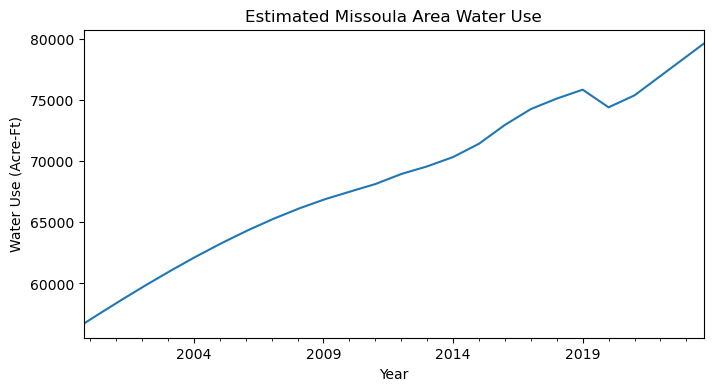
\includegraphics{report_files/figure-pdf/fig-water-use-output-1.png}

}

\caption{\label{fig-water-use}Estimated water use based on the U.S.
Census population data within the Missoula area and an average
consumption of 160 gallons/day/person.}

\end{figure}%

\begin{figure}

\centering{

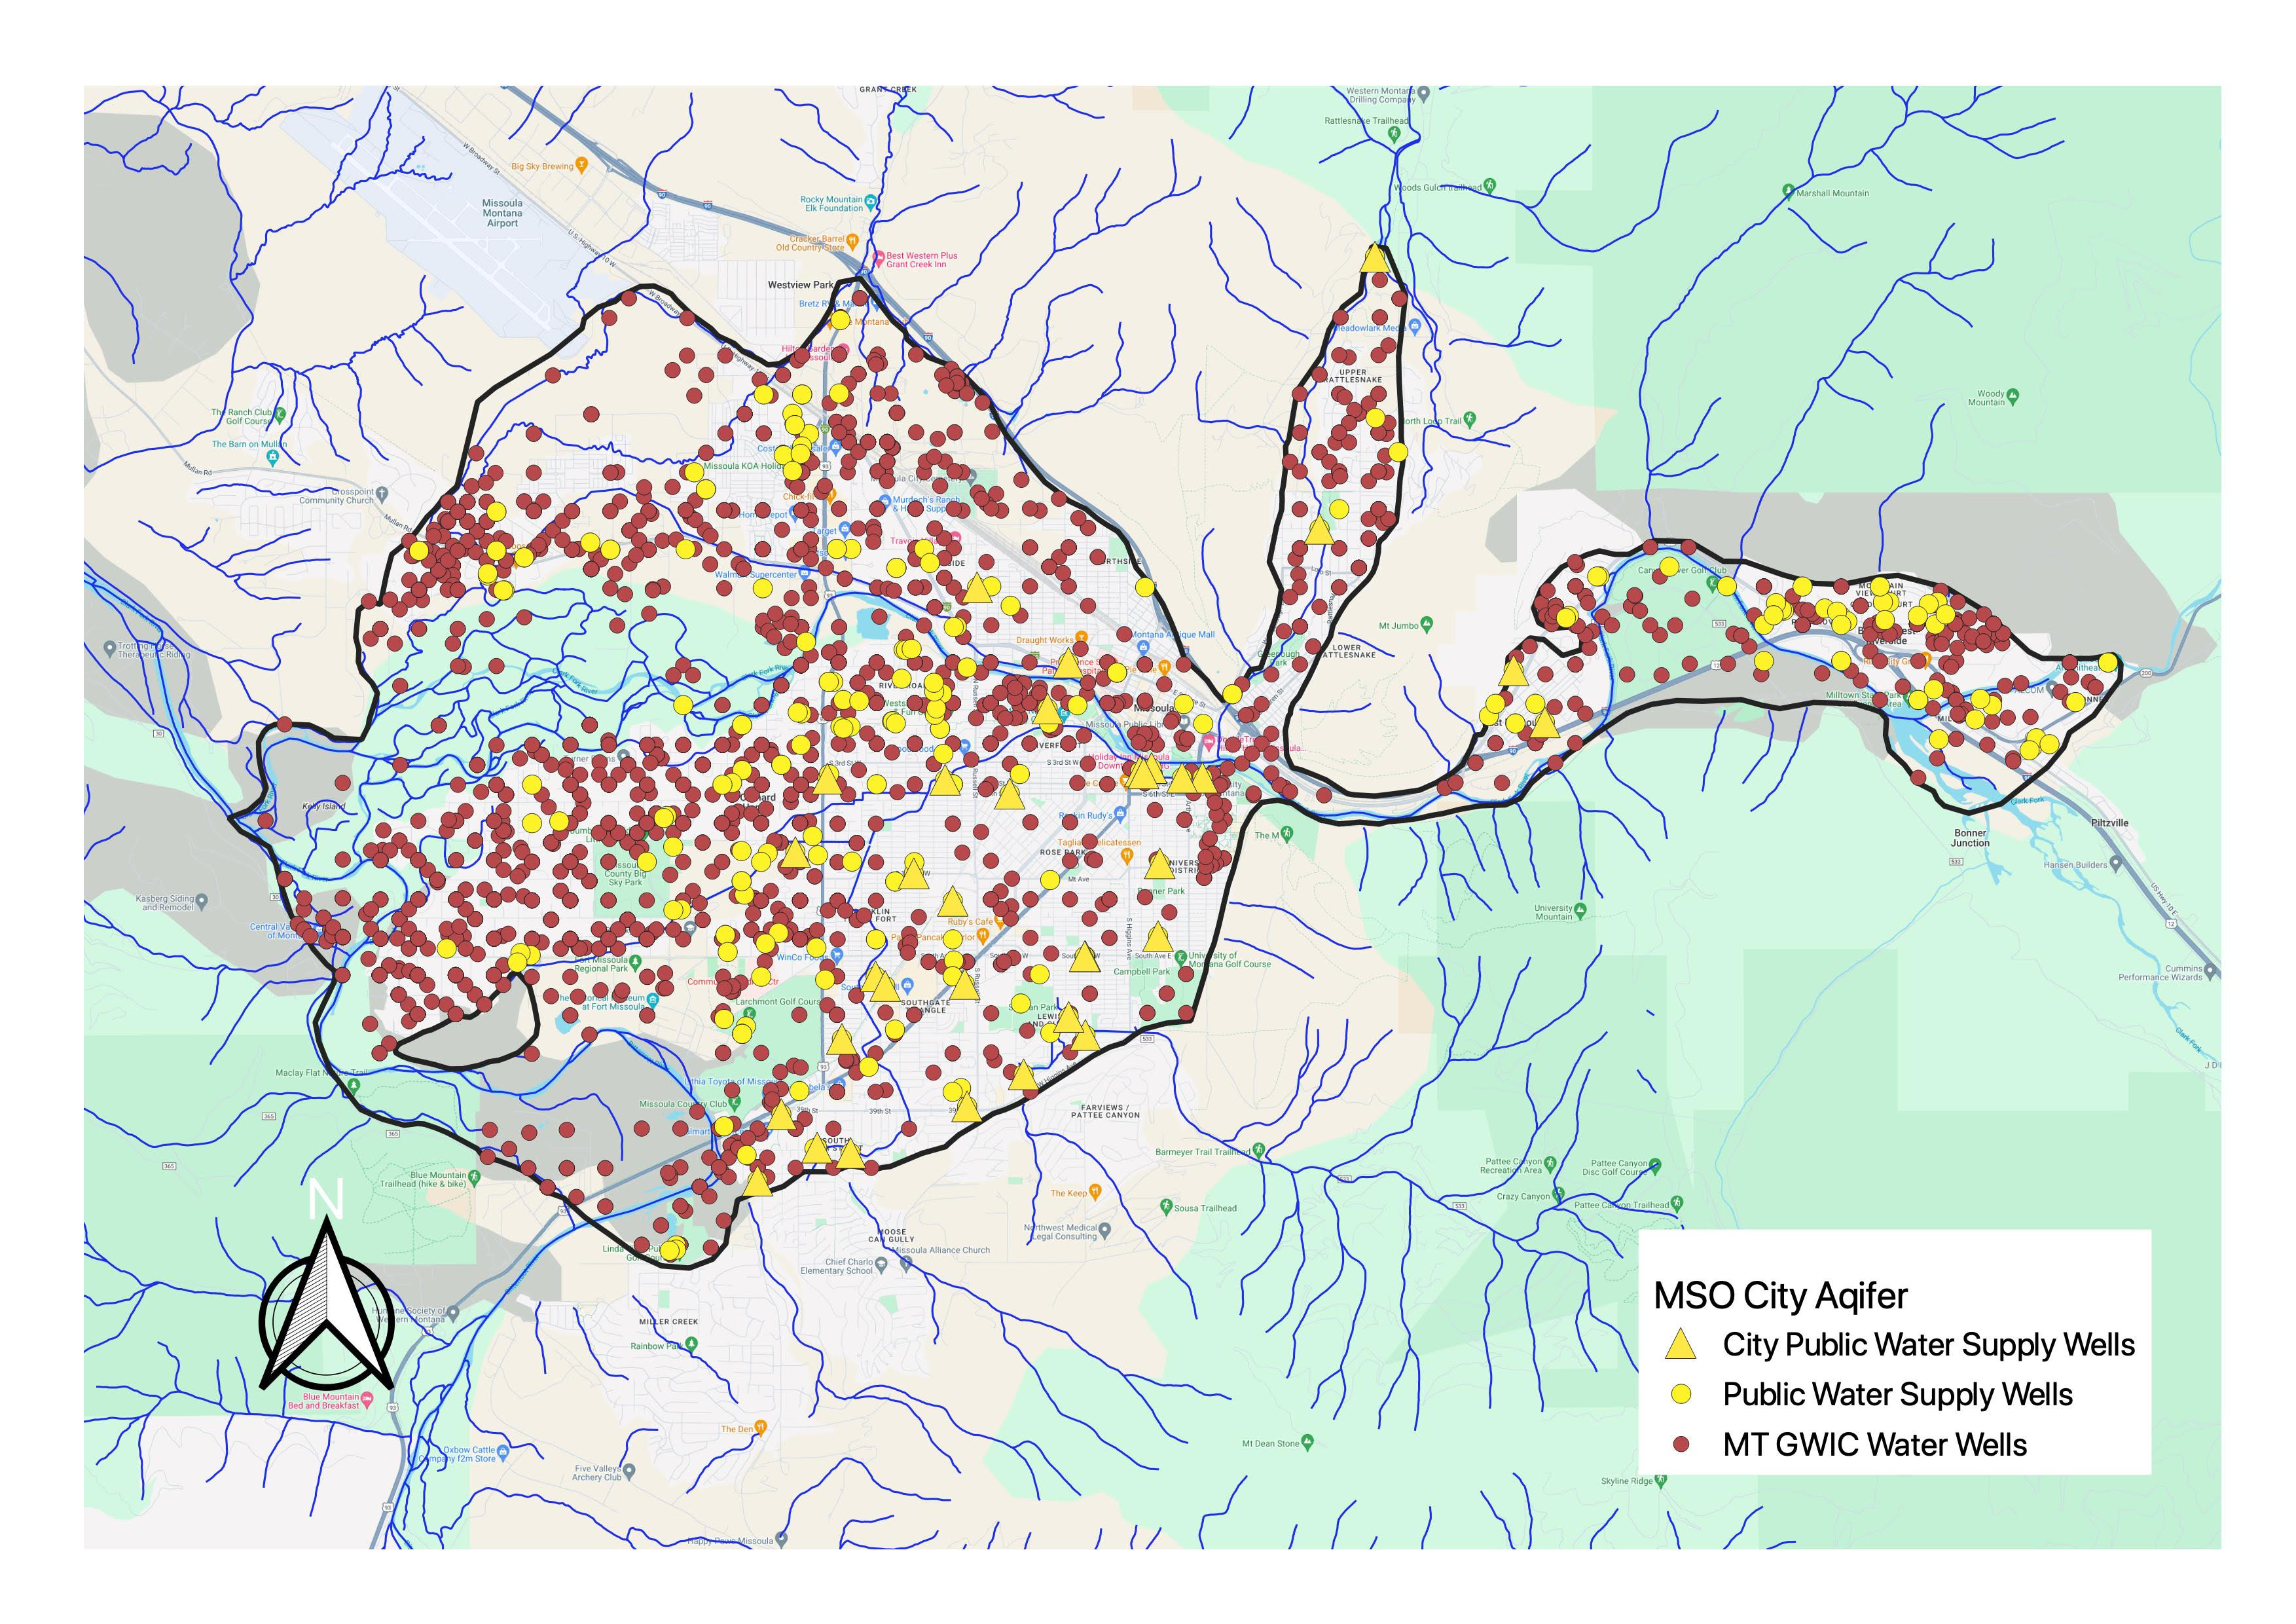
\includegraphics{./images/mso_map_of_all_wells.jpg}

}

\caption{\label{fig-extract-map}All extraction wells within the Missoula
area (eastern Missoula Aquifer).}

\end{figure}%

What if climate change and population growth converge to maximize stress
on the aquifer? While these kinds of scenarios are not determined, they
are all well within the realm of realistic possibilities, perhaps even
probable. Given the overall resilience that we have seen in the past, it
is possible that the aquifer can withstand these stressors and continue
to deliver clean and plentiful potable water to the Missoula community
in perpetuity. However, to date, no one has studied these different
scenarios to make sure that our future water resources are protected. In
this analysis, we first evaluate the long-term historial trends in Clark
Fork River discharge, City of Missoula pumping rates, and Missoula
Aquifer water table depth. In subsequent analyses (not inlcuded in this
preliminary report) we plan to specifically study the impacts of
plausible future scenarios on the Aquifer to identify critical tipping
points and mitigation strategies.

\subsection{Methods}\label{methods}

\subsubsection{Study Area}\label{study-area}

The study area includes the greater Missoula area. Within this region
there are 16 monitoring wells used in the analysis
(Figure~\ref{fig-site-map}).

\begin{figure}

\centering{

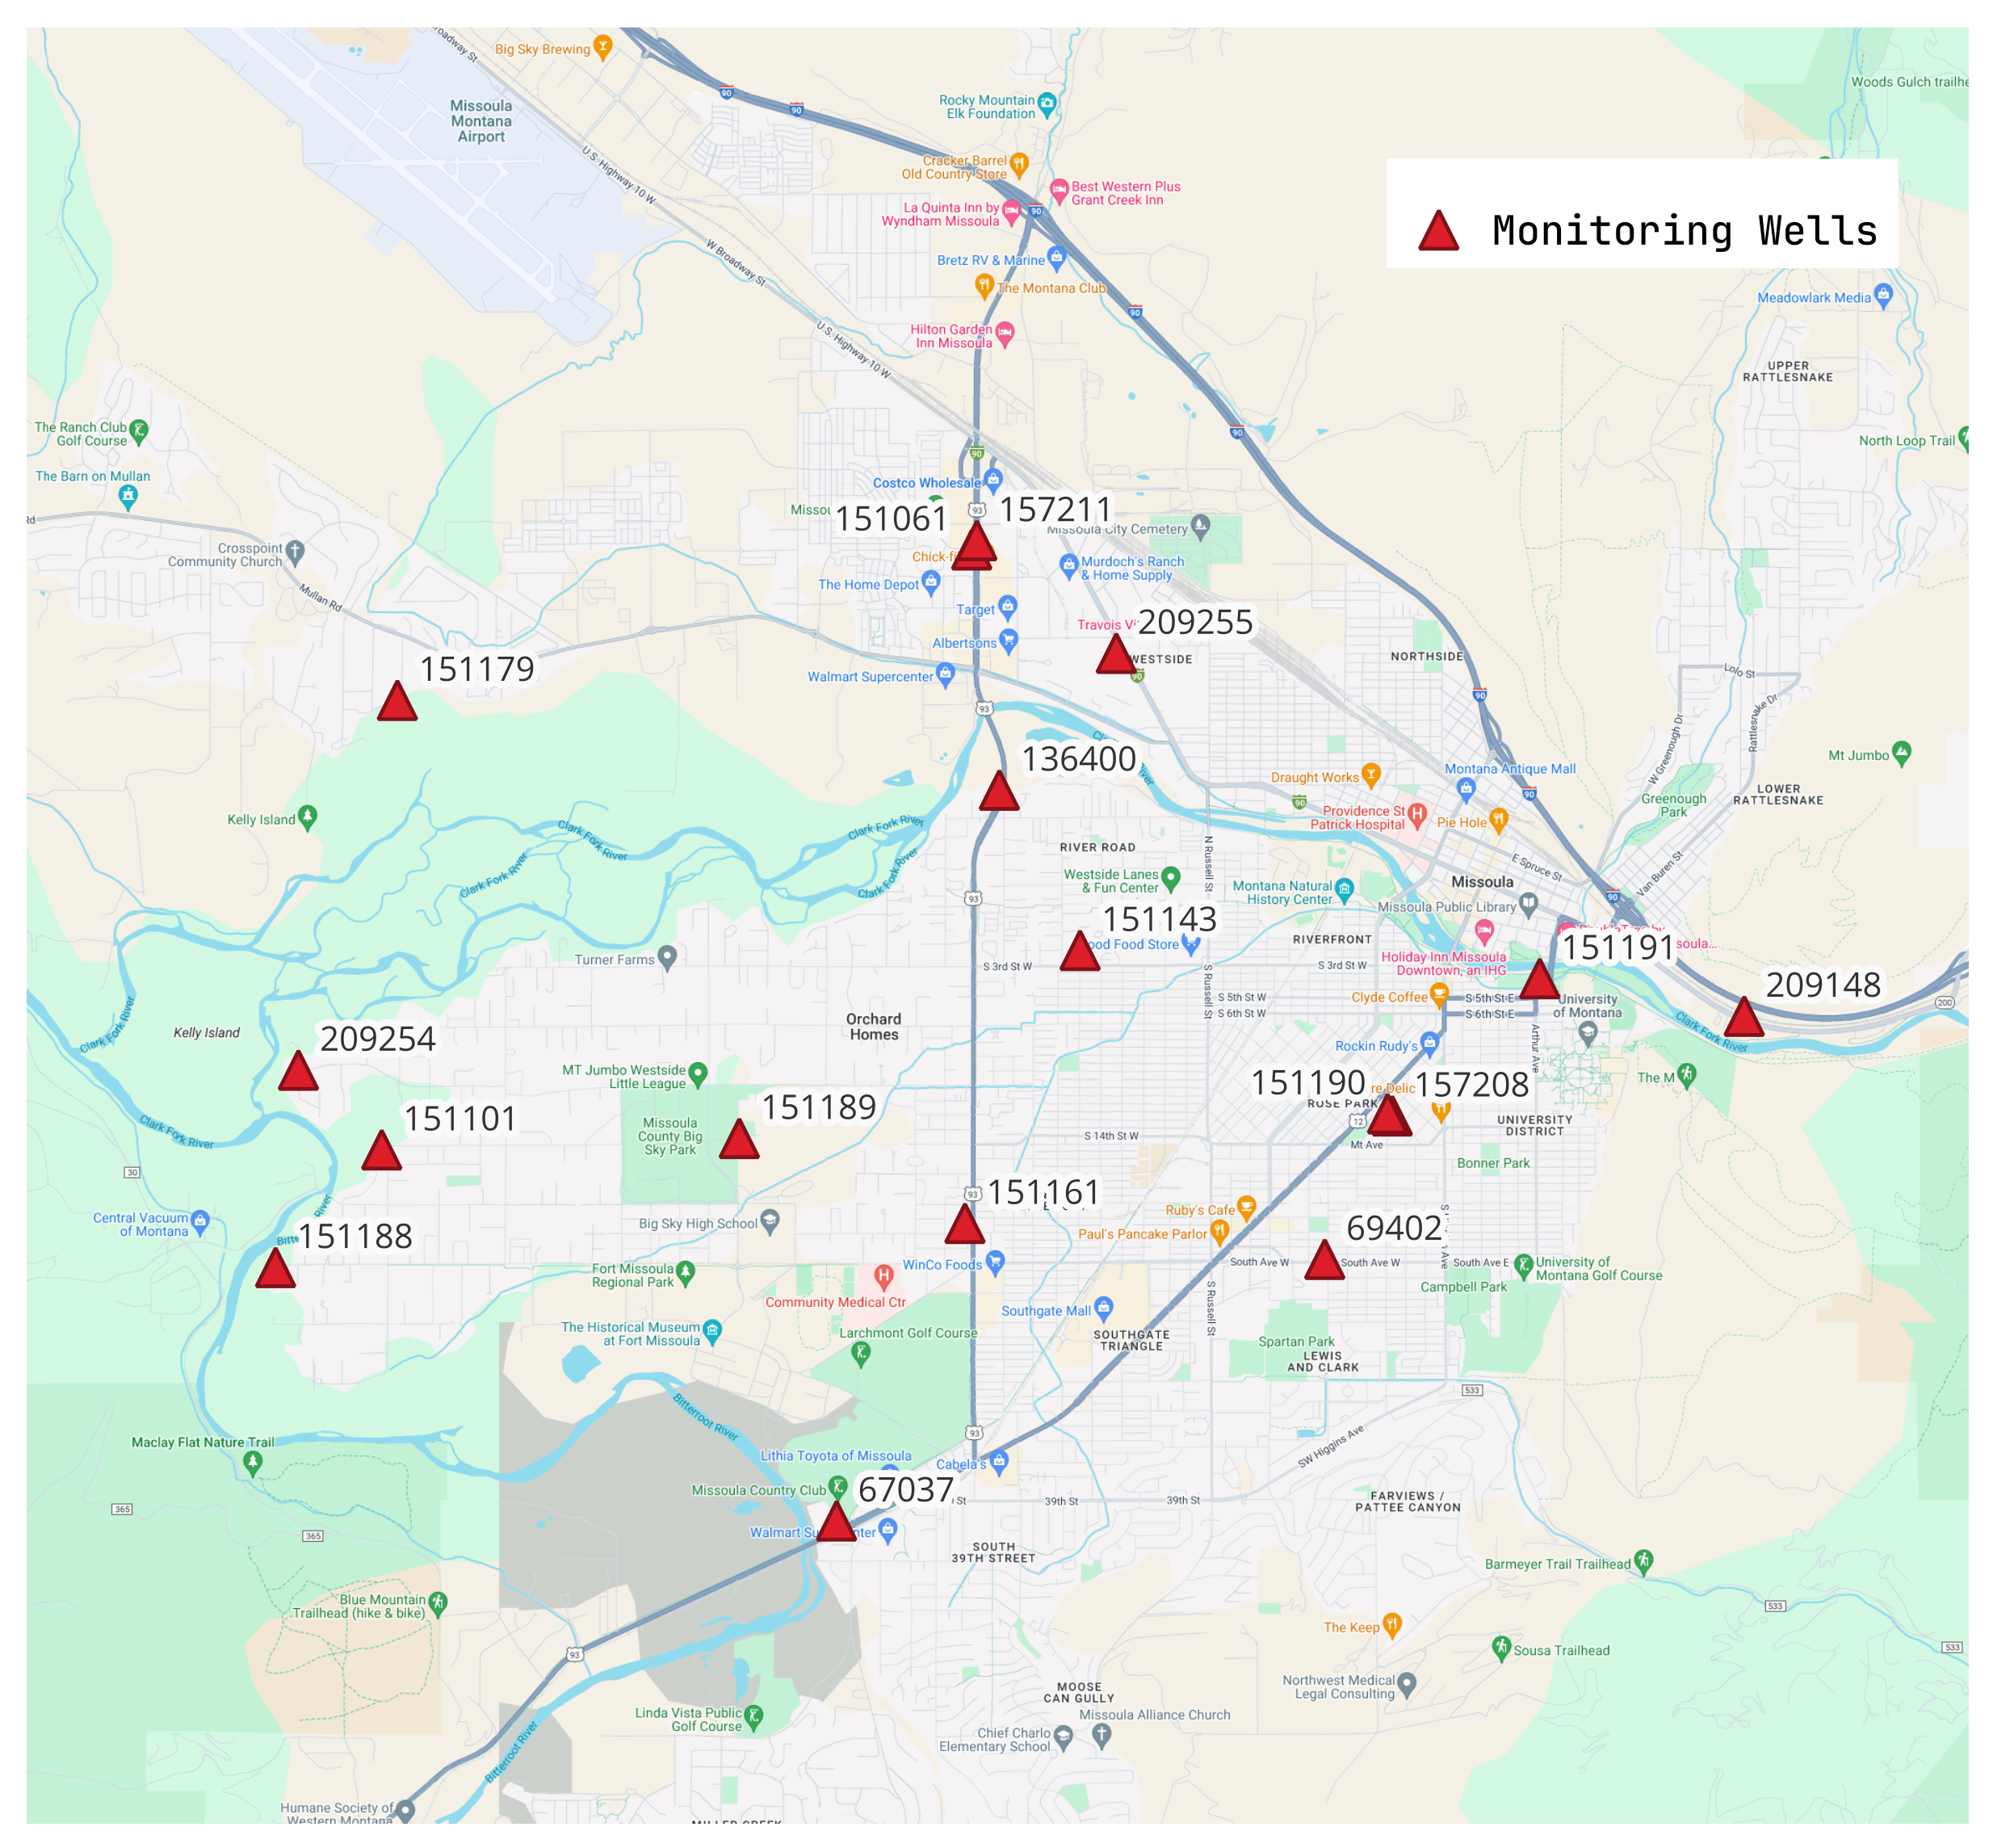
\includegraphics{./images/site_map.png}

}

\caption{\label{fig-site-map}The study site including the 16 monitoring
wells used in the analysis.}

\end{figure}%

\subsubsection{Data Imputation (Gap
Filling)}\label{data-imputation-gap-filling}

The historical groundwater measurements from the 16 monitoring wells
used in our analyses, were taken sporadically and inconsistently over
the study time period (Figure~\ref{fig-gw-imputation}). Therefore, in
order to compare across all sites we needed to fill the data gaps and
resample to monthly average values. We used a two-step approach to gap
fill the data. In the first step we identified the two wells with close
to continuous data (e.g.~151189 and 151190;
Figure~\ref{fig-gw-imputation}). We then used seasonal trend
decomposition using LOESS (STL; Cleveland et al. (1990)) to fill in the
few missing data points of those two wells. In the second step, we
developed a multiple linear regression (MLR) model for each well using
the two complete wells plus the day of year (i.e.~last day of the month)
as independent, predictor variables. We used this MLR model to impute
data into the gaps of each well independently to create consistent
monthly data across all water-years (2000-2023) in each monitoring well
used in the study. We tested several other methods including linear
interpolation, time-based interpolation, MLR using Clark Fork River
flows, and STL by iterating the method 100 times and leaving out 5 known
data points to later predict with the model. The multiple linear
regression imputation method using the two complete wells and day of
year proved to have the best error statistics across the all metrics
(MAE, MSE, RMSE, MAPE, and R-squared;
Table~\ref{tbl-error-stats})\footnote{https://vitalflux.com/mse-vs-rmse-vs-mae-vs-mape-vs-r-squared-when-to-use}.

\begin{figure}

\centering{

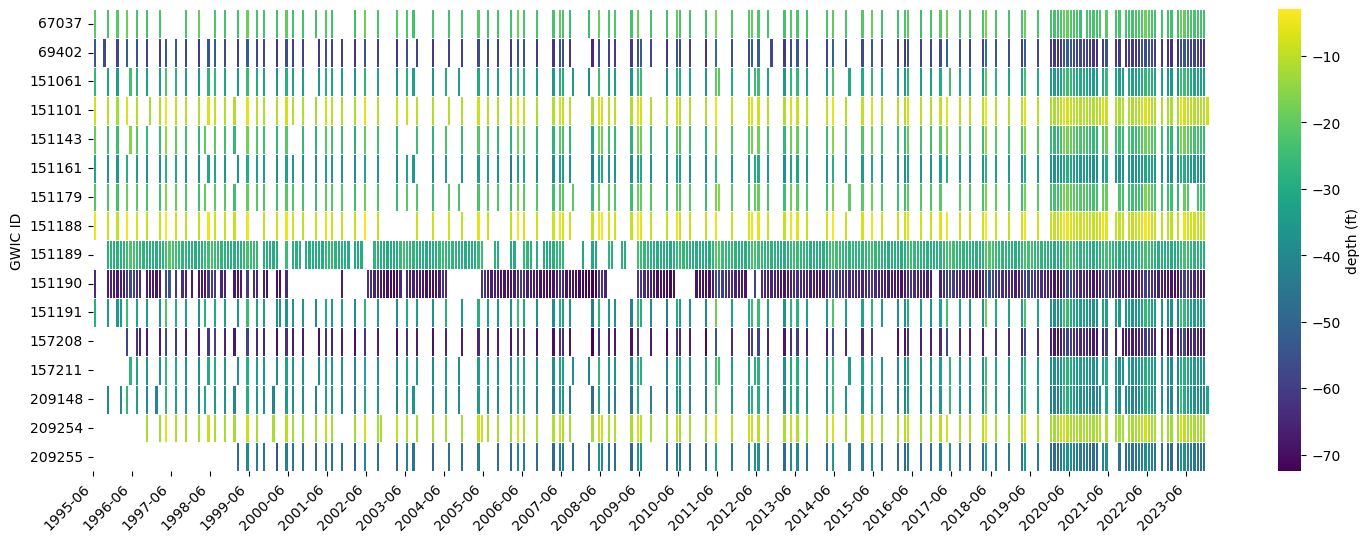
\includegraphics{report_files/figure-pdf/fig-gw-imputation-output-1.png}

}

\caption{\label{fig-gw-imputation}The groundwater monitoring sampling
dates for each well before gap filling. The y-axis is the MT GWIC number
of the well. The vertical lines represent the date sampled for each
well. Color represents the value of the measurement (i.e.~depth below
ground). Since 2020, nearly all the wells have fairly dense records,
missing few months (white areas). Only two wells (151189 \& 151190) have
fairly full records (data for each month of the year). The others have
sparse data in the beginning of the record. We used multiple linear
regression imputation, to fill these gaps based on relationships between
water table depth and the day of the year and the two wells with the
most complete data. This resulted in a continuous monthly dataset from
Oct 1999 through Sep 2023.}

\end{figure}%

\begin{longtable}[]{@{}llllll@{}}

\caption{\label{tbl-error-stats}Error statistics from the data
imputation methods tested. For this study we used the STL Decomposition
to fill data in the two most complete wells and then used the Well (MLR)
Regression method using those two wells and day of year to build models
for each well and use those models to gill gaps in the data record.}

\tabularnewline

\toprule\noalign{}
& MAE & MSE & RMSE & MAPE & R\^{}2 \\
\midrule\noalign{}
\endhead
\bottomrule\noalign{}
\endlastfoot
Linear Interpolation & 2.4923 & 13.8497 & 3.7215 & 10.5845 & 0.9556 \\
STL Decomposition & 1.3017 & 3.9748 & 1.9937 & 5.4697 & 0.9873 \\
Time Interpolation & 2.4703 & 13.7026 & 3.7017 & 10.5757 & 0.9563 \\
Q and DOY Regression & 1.6086 & 4.9560 & 2.2262 & 6.1077 & 0.9843 \\
Well Regression & 0.9365 & 1.9474 & 1.3955 & 4.5326 & 0.9929 \\

\end{longtable}

\subsection{Historical Analysis}\label{historical-analysis}

\subsubsection{Clark Fork River}\label{clark-fork-river}

The Clark Fork River serves as the main source for aquifer recharge in
the Missoula Valley (Tallman 2005). While other inputs exist, we focus
almost exclusively on the Clark Fork due to the overall magnitude
relative to other inputs. A seasonal decomposition using LOESS
(Cleveland et al. 1990) shows that there has been a consistent
increasing trend in monthly average flows over the study period
(2000-2023; Figure~\ref{fig-cfr-stl}). Change was steepest through 2011
and then flattened through the rest of the record. In addition, as
expected, there is a strong seasonality component with peak flows coming
in late spring and baseflows in late summer and early fall. The
magnitude of seasonality is increasing, with the peaks getting higher
and the troughs getting lower -- suggesting an increasing trend in
interannual variability through time.

\begin{figure}

\centering{

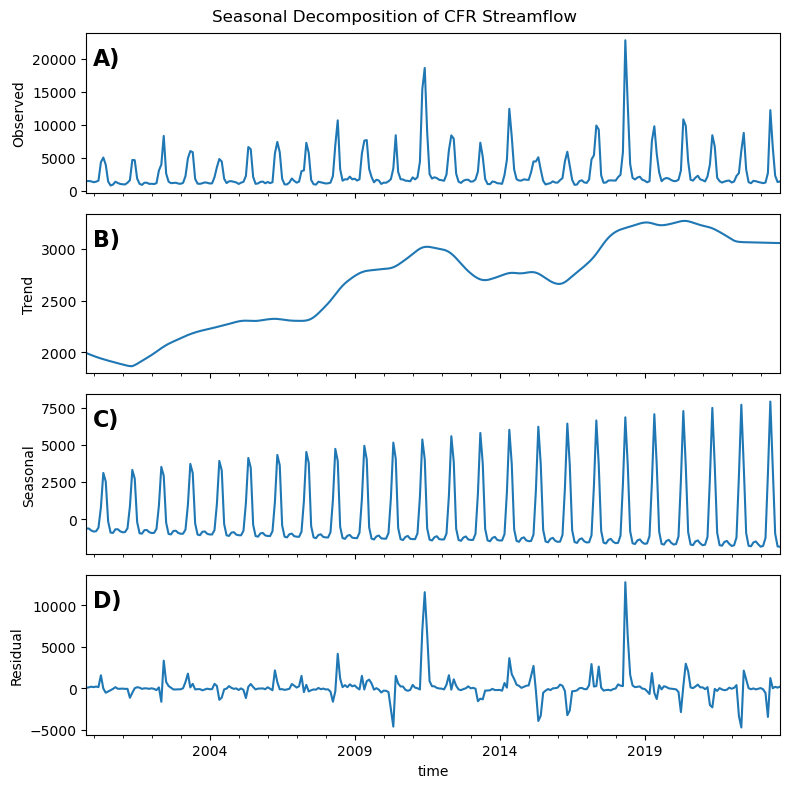
\includegraphics{report_files/figure-pdf/fig-cfr-stl-output-1.png}

}

\caption{\label{fig-cfr-stl}Seasonal decomposition of the Clark Fork
River monthly streamflows. The top panel (A) is the full stremflow
signal--the mean daily discharge for each month from 2000 to 2023. The
second panel (B) shows the trend over the time period with other signals
removed. The third panel (C) is the seasonal signal without the trend.
And the bottom panel (D) is the remainder of the signal no catpured by
the trend and seasonal components.}

\end{figure}%

We further investigate the trend of the Clark Fork River flows using a
Mann-Kendall statistical significance test (Mann 1945; Kendall 1975),
which avoids assumptions of normality and independence. The results
indicate a statistically significant (\(p<0.05\)) increasing trend of 24
cfs/month. We further break down the trend analysis into seasons: winter
(December, January, February), spring (March, April, May), summer (June,
July, August), and fall (September, October, November)
(Figure~\ref{fig-cfr-seas-trends}). All four seasons have increasing
trends, although the summer season's trend is not statistically
significant at the \(p<0.05\) level. The spring runoff trend is by far
the strongest, representing a slope 113 cfs/season. Spring is the season
where most of the recharge from the Clark Fork River to the Missoula
Aquifer occurs (Tallman 2005).

\begin{figure}

\centering{

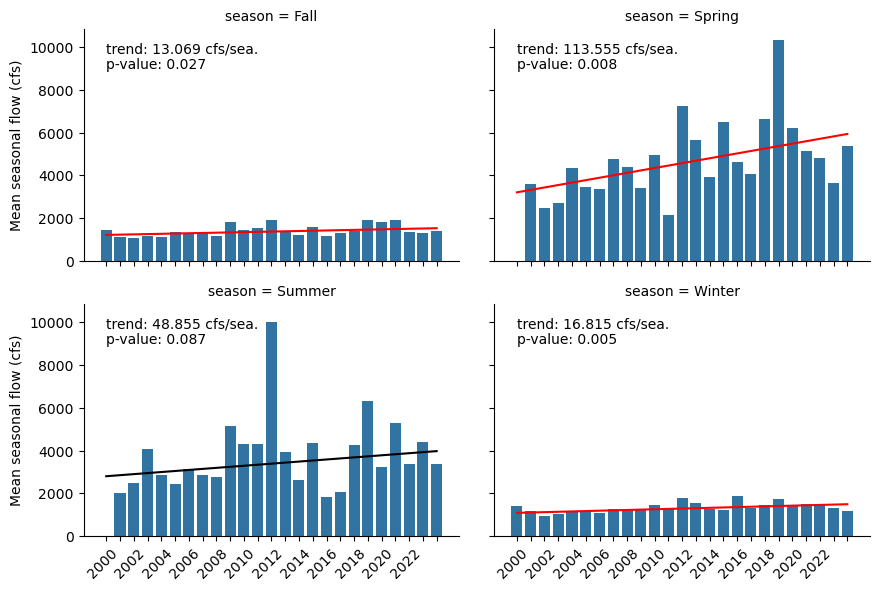
\includegraphics{report_files/figure-pdf/fig-cfr-seas-trends-output-1.png}

}

\caption{\label{fig-cfr-seas-trends}Seasonal trends for Clark Fork River
flows. Red line indicate a statistically significant (\(p<0.05\)) trend;
black line indicates a non- statistically significant
(\$\textgreater=0.05) trend. The amount of the trend in cfs/season and
p-values are shown on each panel.}

\end{figure}%

\subsubsection{Groundwater Table Depth}\label{groundwater-table-depth}

We evaluated trends in groundwater table depth for each of the 16 wells
within the study site using the Mann-Kendall test. All 16 wells have
statistically significant increasing trends and strong seasonality,
similar to the Clark Fork River streamflow (Figure~\ref{fig-gw-trends}).
On average, there has been approximately a 1.9 foot increase in
elevation of the water table over the period of record. Trends and
timeseries data are very similar across all the sites, supporting
previous studies showing high transmissivity throughout the aquifer
(Tallman 2005; Miller 1991).

\begin{figure}

\centering{

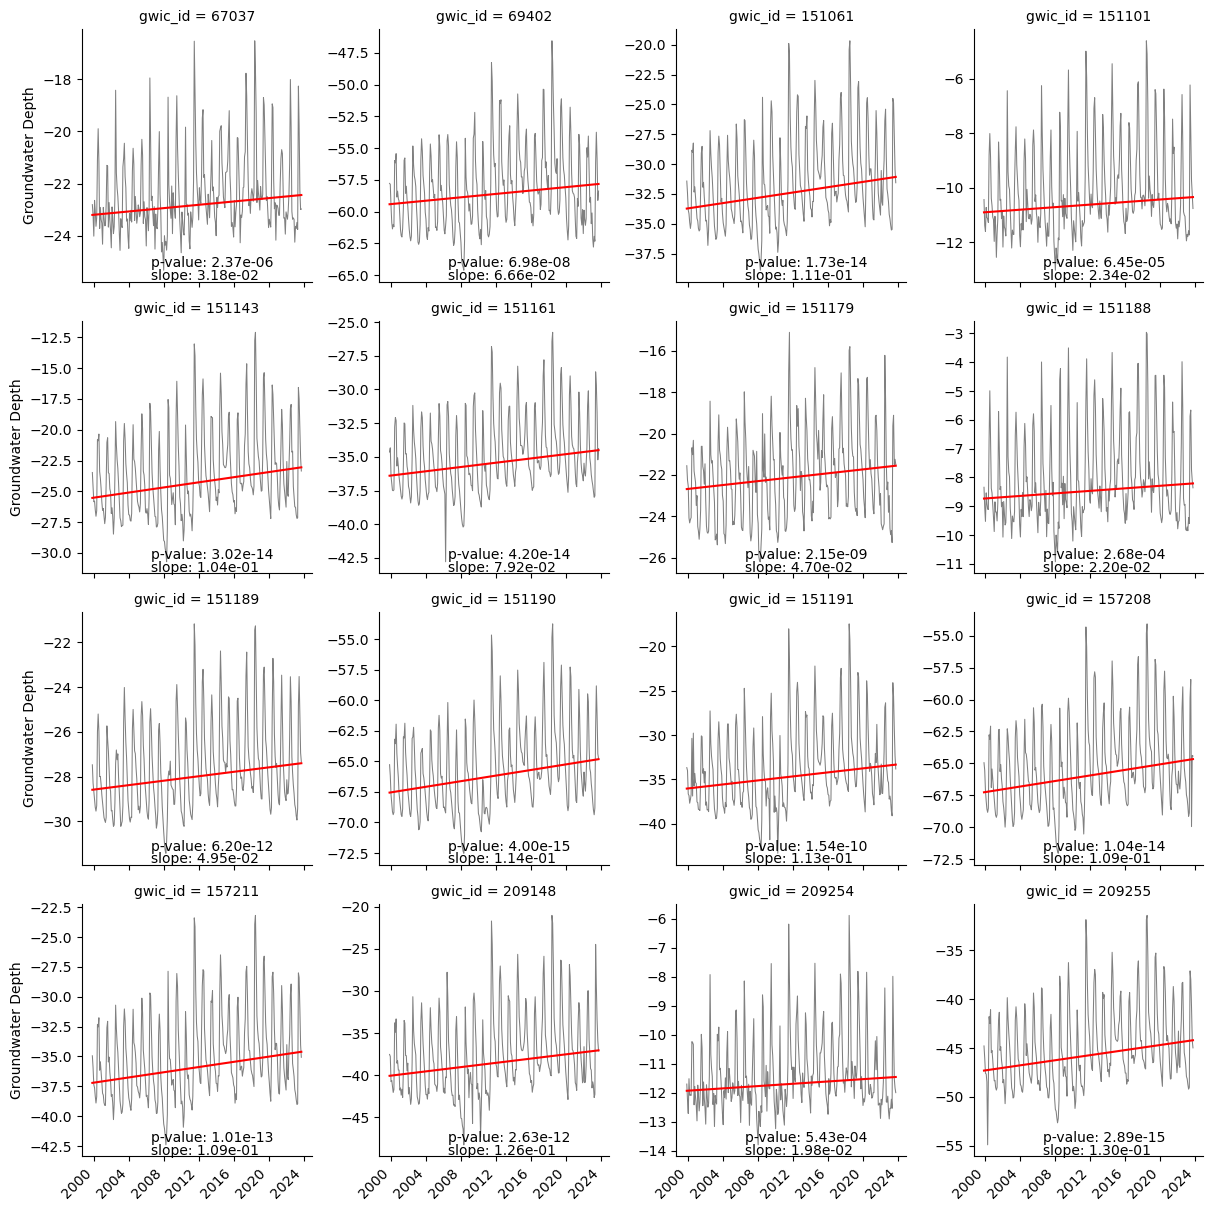
\includegraphics{report_files/figure-pdf/fig-gw-trends-output-1.png}

}

\caption{\label{fig-gw-trends}Trends in groundwater depth for the 16
wells within the study area. Red line indicates a statistically
significant trend (\(p<0.05\)).}

\end{figure}%

Additionally, we calculated the 10th, 50th, and 90th quantile regression
lines to show trends in lower, median, and upper groundwater values,
respectively (Figure~\ref{fig-gw-quantreg}). The changes in the 10th and
90th quantiles can be thought of as changes in the late Summer and early
Spring since those are the times of year when groundwater elevations are
at a minimum and maximum, respectively. The results show strong
increasing trends in the 90th quantile, suggesting that increases in
peak recharge events in the Spring are largely driving the overall trend
in the groundwater. Median and lower quantiles show less of an
increasing trend. The difference in trends between the 90th and 10th
percentile also suggest an overall increase in interannual variability
throughout the time period, similar to the seasonality trend in the
Clark Fork River seasonal decomposition analysis
(Figure~\ref{fig-cfr-stl}).

\begin{figure}

\centering{

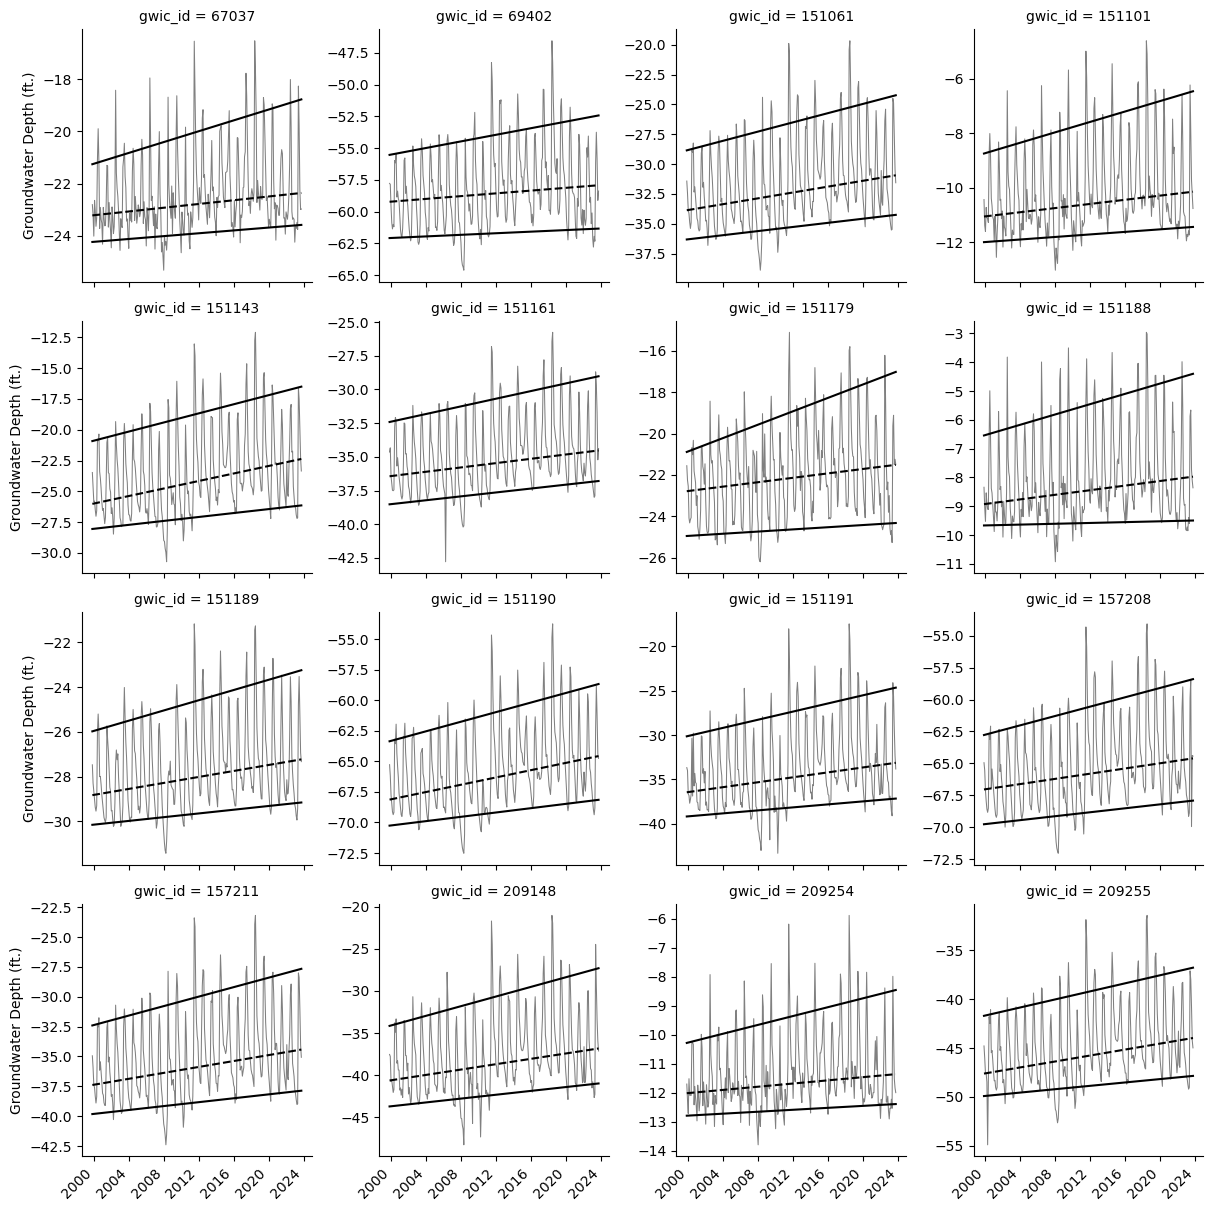
\includegraphics{report_files/figure-pdf/fig-gw-quantreg-output-1.png}

}

\caption{\label{fig-gw-quantreg}Upper (90th percentile), median (50th
percentile, dashed), and lower (10th percentile) trends in groundwater
data. The 90th percentile trends are consistently the largest,
suggesting increases in peak recharge events and interannual
variability.}

\end{figure}%

\subsubsection{Groundwater Withdrawals}\label{groundwater-withdrawals}

To understand the relationship and patterns of groundwater levels, Clark
Fork streamflow, and Missoula City pumping rates, we normalize all
monthly values to be between zero and one (Figure~\ref{fig-norm-ts}). We
average the normalized groundwater depths across all wells to get a
representative groundwater signal to compare to river flows and pumping
rates. The signals are remarkably aligned in their seasonality.
Essentially, the City is increasing their pumping at the same time
streamflow, and thus groundwater, are at their maximum. This is an
opportunitistic situation and one that should be monitored closely if
streamflow timing were to shift due to changes in snowpack runoff, as
projected by climate change studies (Whitlock et al. 2017). The main
difference in these three signals is the lagged decrease in groundwater
levels in comparison to the river and pumping rate. Groundwater tends to
drop much slower than the two independent variables, suggesting there is
some storage effect in the unconfined aquifer. This may help to mitigate
some future shifts in peak streamflow if they were to occur.

\begin{figure}

\centering{

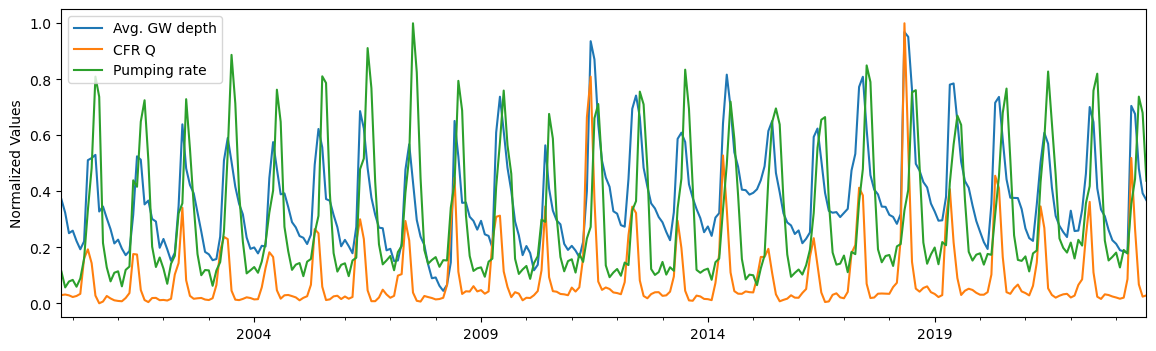
\includegraphics{report_files/figure-pdf/fig-norm-ts-output-1.png}

}

\caption{\label{fig-norm-ts}Normalized timeseries values for average
groundwater depth (blue), Clark Fork River streamflow (orange), and
Missoula City pumping rates (green). All values are monthly averages.}

\end{figure}%

We perform a seasonal decomposition analysis using LOESS on the City
pumping rate time series (Cleveland et al. 1990). Similar to the Clark
Fork River flows and groundwater level, the City pumping rate has a
slight increasing trend and strong seasonality over the study time
period (Figure~\ref{fig-pumping-stl}). While the overall trend is
increasing, there are three smaller trends that are distinct across the
time period. From 2000 to 2008 the pumping rate increases, then from
2009 to 2015 the pumping rate decreases, followed by another strong
increasing trend from 2016 to 2023. The effects of these inflection
points in the pumping rate trends are explored in further detail later
in this section.

\begin{figure}

\centering{

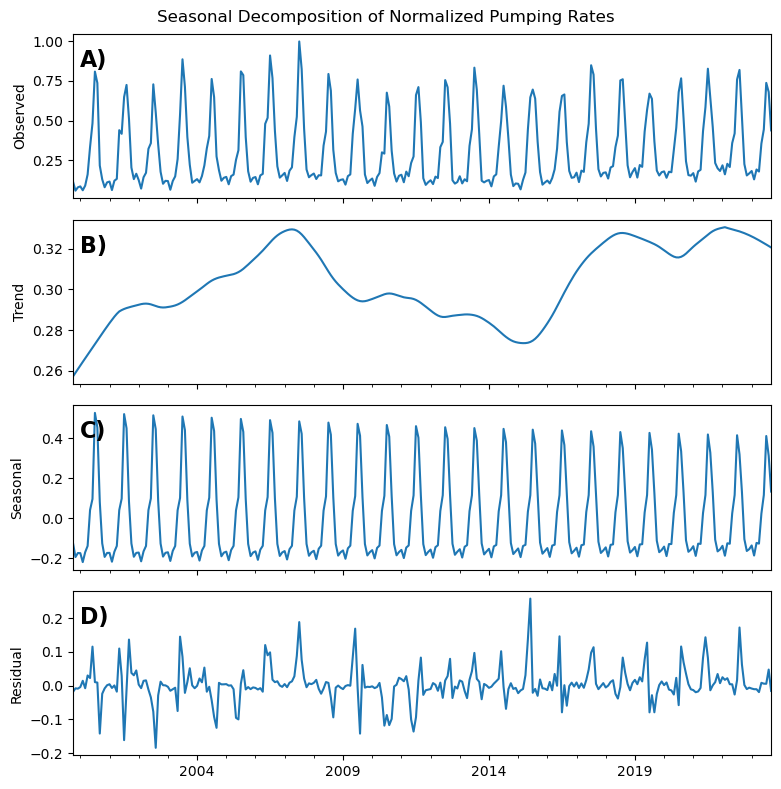
\includegraphics{report_files/figure-pdf/fig-pumping-stl-output-1.png}

}

\caption{\label{fig-pumping-stl}The seasonal decomposition using LOESS
of the City of Missoula pumping rates. Panel A) is the combined signal,
panel B) is the trend, panel C) is the seasonality, and panel D) is the
residual after trend and seasonality are removed.}

\end{figure}%

The most recent 10 water-years (2014-2023) provide an interesting case
study. Over this time period, pumping rates have strongly increased
(Figure~\ref{fig-pumping-stl} B) and river flows have remained around
the same (slight increase; Figure~\ref{fig-cfr-stl} B), yet the
groundwater trends from all of the wells have decreased over this time
period. Furthermore, most of these decreases are statistically
significant (Figure~\ref{fig-gw-recent}). This suggests that there are
likely other factors (i.e.~groundwater witdrawals), beyond the Clark
Fork River flows, influencing groundwater levels.

\begin{figure}

\centering{

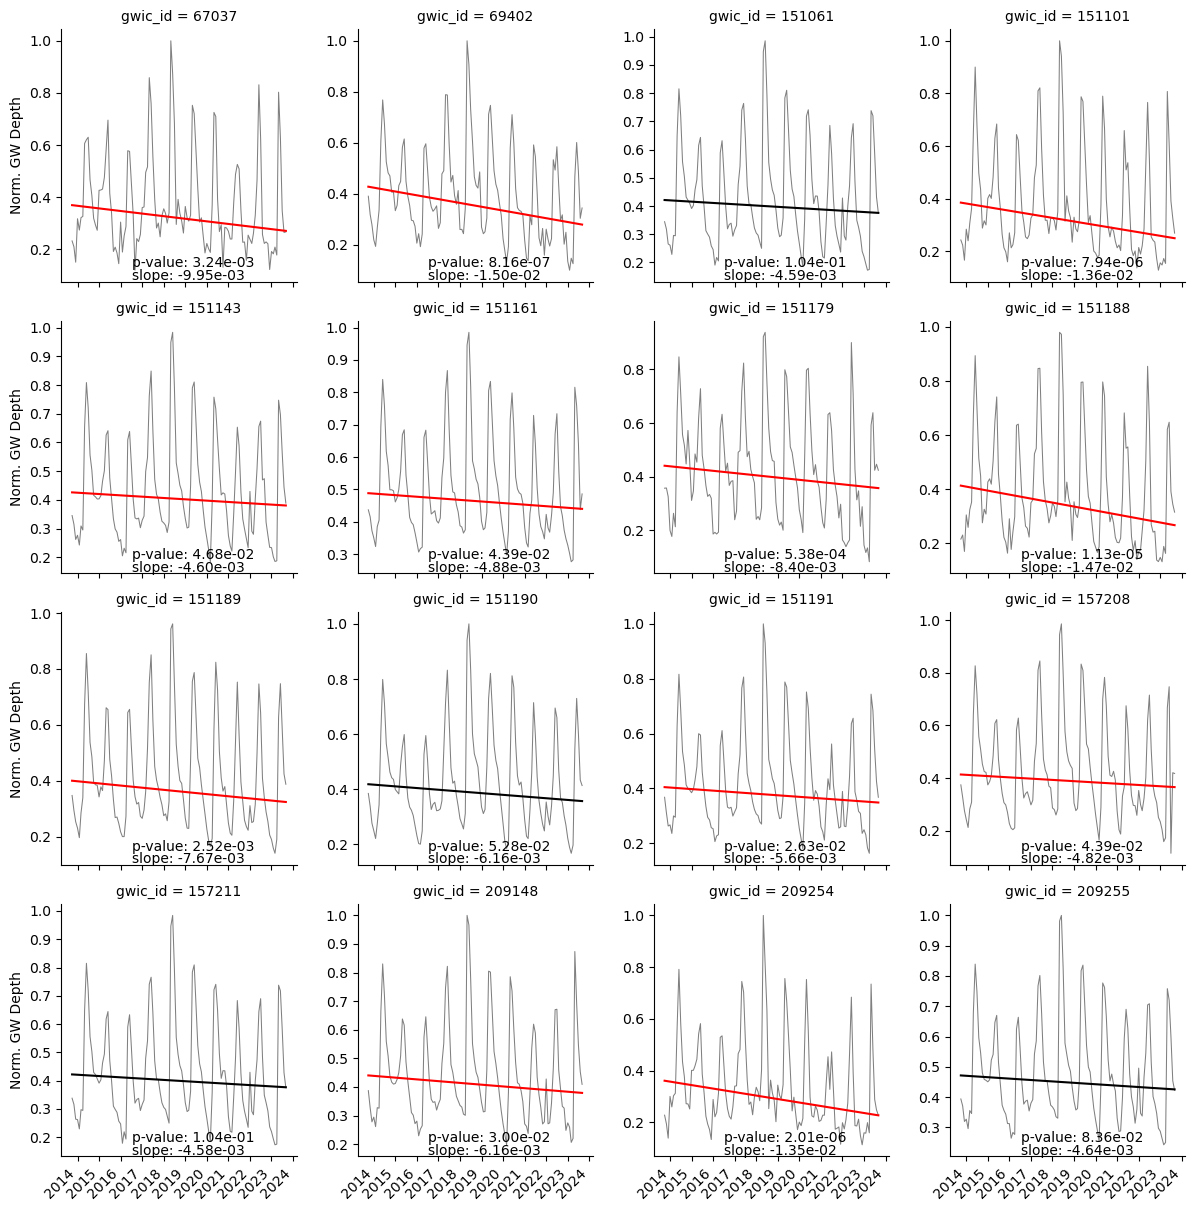
\includegraphics{report_files/figure-pdf/fig-gw-recent-output-1.png}

}

\caption{\label{fig-gw-recent}The most recent 10-years of groundwater
level data with trends (significant and non-significant).}

\end{figure}%

In order to understand how withdrawals may be impacting groundwater
levels over the entire time period, we remove the normalized trend in
river flow from the groundwater signal at all wells
(Figure~\ref{fig-gw-qremoved}). This is, we produce a time series of
what ground water depth would look like if the increasing trend of the
Clark Fork River flow was removed. This allows us to focus on what the
groundwater level would be doing if there was no trend in recharge from
the river. With the river flow trend removed, increasing trends in
groundwater elevation are reduced in all 16 wells. Five of the 16 lose
statistical significance and one shifts from increasing to decreasing;
although not statistically significant. This suggests that if the river
flows were not increasing over this time period, groundwater trends
would not have the same strong increasing trend that we see in the
record. Thus, it appears that there is a potential for the river to mask
the impact of City pumping rates and that without the increasing
streamflow we may see much different behavior in the aquifer water
table.

\begin{figure}

\centering{

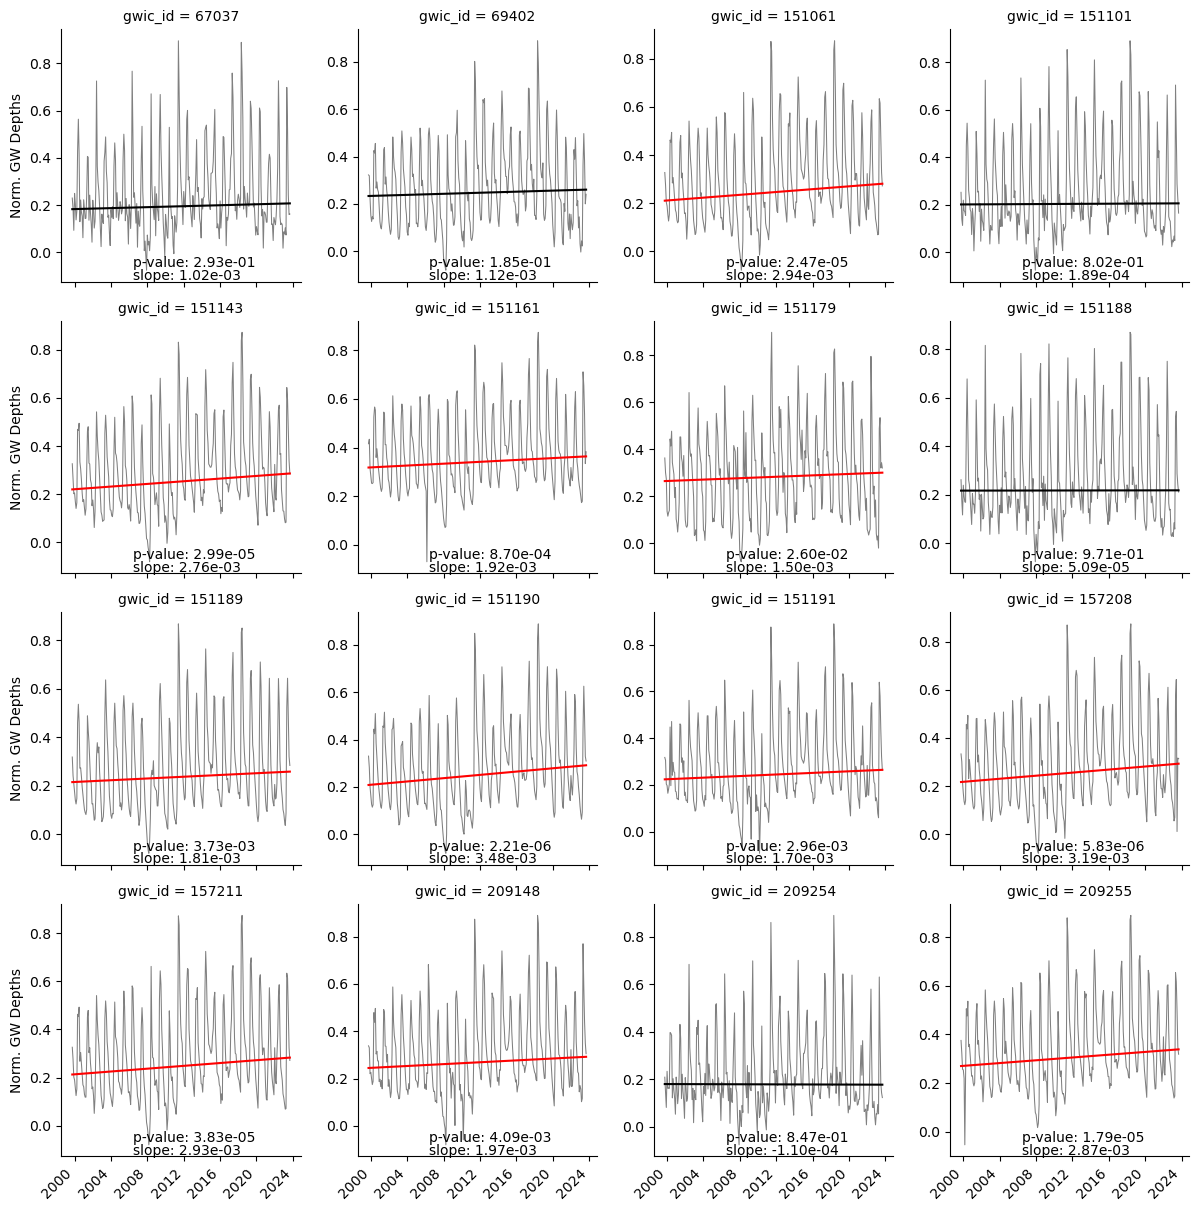
\includegraphics{report_files/figure-pdf/fig-gw-qremoved-output-1.png}

}

\caption{\label{fig-gw-qremoved}Trends in groundwater depth after the
normalized Clark Fork River has been removed.}

\end{figure}%

In reality there is not a single long-term trend in pumping rates, but
instead, three short-term trends (Figure~\ref{fig-pumping-stl} B). The
first trend is increasing from 2000 to 2008, the next trend is
decreasing from 2009 to 2015, and the last trend is increasing from 2016
to 2023. With the effects from the Clark Fork River trend removed we
explore the trends in the average normalized groundwater elevation and
pumping rates over these three distinct time periods
(Figure~\ref{fig-gw-pr-trends}). In the first time period (2000-2008)
groundwater elevation decreases as pumping rates increase. In the second
time period (2009-2015) groundwater elevation increases as pumping rates
decrease. And in the third time period (2016-2023) groundwater elevation
decreases as pumping rates increase. All trends in both the groundwater
and pumping rates are statistically significant. This analysis suggests
that City pumping rates can impact the groundwater level in
statistically signifacant ways. Therefore, without the recent increase
in streamflow, we might be experiencing very different trends in the
Missoula Aquifer level. If trends in Clark Fork River flows were to
reverse (or even stabilize) and pumping rates were to continue to
increase, it is possible that an unsustainable condition in the
groundwater level could be created.

\begin{figure}

\centering{

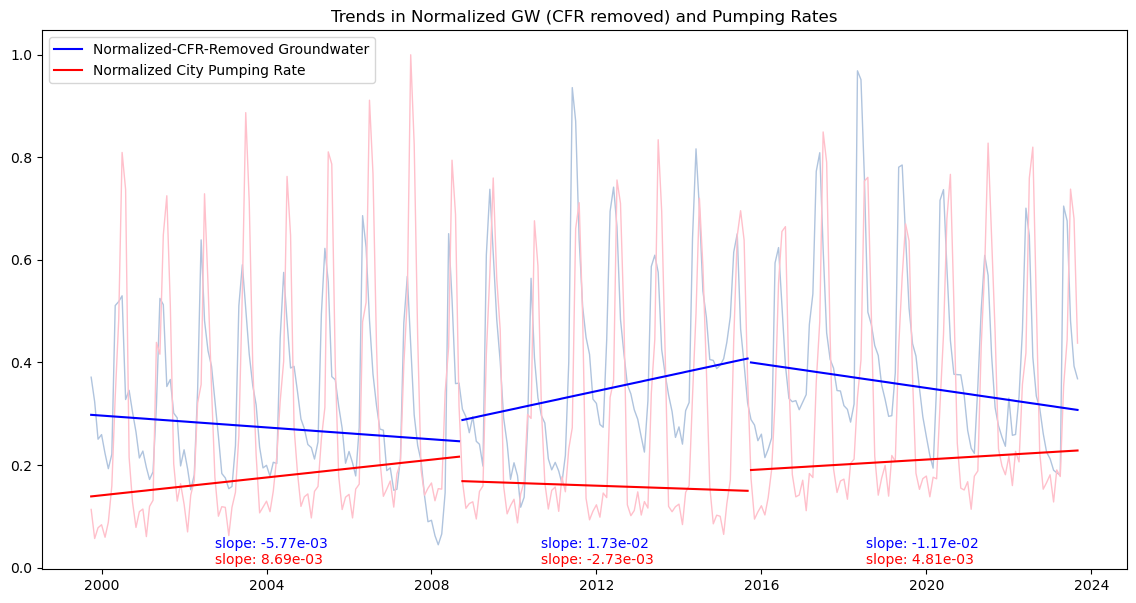
\includegraphics{report_files/figure-pdf/fig-gw-pr-trends-output-1.png}

}

\caption{\label{fig-gw-pr-trends}Trends in normalized average
groundwater depth after CFR trend removed from the data (i.e.~corrected;
blue) and trends in normalized Missoula City pumping rates (red) over
three different time periods: (1) 2000--2008, (2) 2009--2015, and (3)
2016--2023. These time periods were chosen to correspond with the
inflection points of change illustrated in Figure~\ref{fig-pumping-stl}.
All trends are statistically significant at the \(p<0.05\) level.}

\end{figure}%

The timing and magnitude of City pumping rates provide a general signal
of the overall groundwater demand in the Missoula area. We compare these
pumping rates to the population and average monthly daily maximum
temperature to determine what is driving the seasonality and trends in
Missoula groundwater demand (Figure~\ref{fig-pr-pop-temp}). Population
was estimated using U.S. Census data.\footnote{https://www.census.gov/programs-surveys/popest.html}
Average monthly daily maximum temperature was estimated using the
meteostat Python library (Lambrecht 2024) which averages values from the
surrounding weather stations. While the increasing trend in population
is hard to see in the pumping rates data, the seasonality of temperature
appears to be highly correlated.

\begin{figure}

\centering{

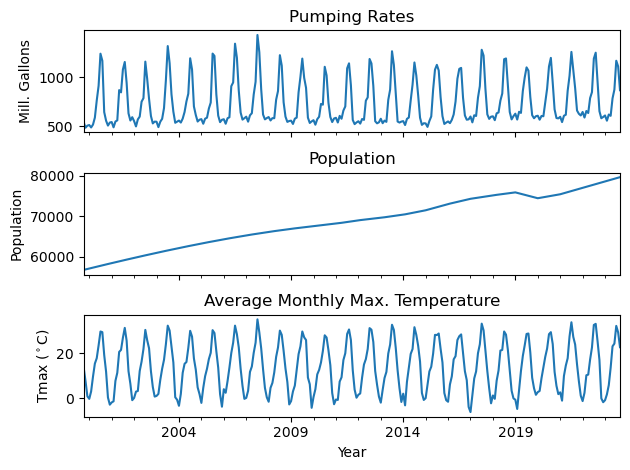
\includegraphics{report_files/figure-pdf/fig-pr-pop-temp-output-1.png}

}

\caption{\label{fig-pr-pop-temp}Timeseries comparison between City
pumping rates, Missoula population, and average monthly daily maximum
temperature.}

\end{figure}%

We analyze the relationships between pumping rates (i.e.~groundwater
demand), population, and maximum temperature using ordinary least
squares multiple linear regression (MLR) analysis. This analysis shows
how much the two independent variables (population and temperature)
explain the variation in the dependent variable (demand). Figure
Figure~\ref{fig-pop-temp-scatter} illustrates the relationship of
pumping rate with population and temperature. We square the temperature
variable to eliminate the exponential relationship and make it linear.
From observing these two scatter plots it is evident that temperature
has a much stronger positive correlation with pumping rates, although
there does appear to be a smaller, positive correlation between pumping
rates with population.

\begin{figure}

\centering{

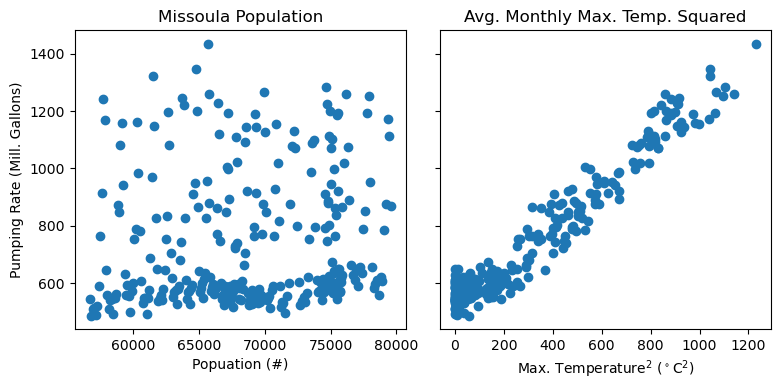
\includegraphics{report_files/figure-pdf/fig-pop-temp-scatter-output-1.png}

}

\caption{\label{fig-pop-temp-scatter}Scatter plots of the City pumping
rates with population and average monthly maximum temperature squared.
Temperature values were squared in order to transform the exponential
relationship to linear.}

\end{figure}%

We develop our MLR model using both population and squared maximum
temperature as predictor variables. The significance of these variables
in explaining pumping rate is show in Table~\ref{tbl-demand-mlr}. The
results suggest that both population and temperature are statistically
significant predictors at the \(p<0.05\) level. In addition, this model
has an \(R^2 = 0.949\), which means that the combination of population
and temperature can explain approximately 95\% of the variance in City
pumping rates. Given the strong the relationship with temperature, we
also explored a MLR with only temperature as a predictor (results not
shown). This model has an \(R^2 = 0.948\), only slighly lower than the
model that includes population, suggesting that pumping rates are highly
dependent on temperature. We did check to see if the model with
temperature alone was better in terms of parsimony but the results (not
shown) suggest that population is worth adding to the model.

\begin{table}

\caption{\label{tbl-demand-mlr}Results from the MLR show key metrics for
population, temperature, and the constant term. The main metric to
consider is \(P>|t|\) which is equivalent to the p-value used in other
statistical tests. Here, population and temperature are both considered
statistically significant at the \(p<0.05\) level.}

\centering{

\begin{center}
\begin{tabular}{lcccccc}
\toprule
                 & \textbf{coef} & \textbf{std err} & \textbf{t} & \textbf{P$> |$t$|$} & \textbf{[0.025} & \textbf{0.975]}  \\
\midrule
\textbf{Const.}  &     435.5509  &       34.550     &    12.606  &         0.000        &      367.545    &      503.557     \\
\textbf{Pop.}    &       0.0014  &        0.001     &     2.786  &         0.006        &        0.000    &        0.002     \\
\textbf{Temp.^2} &       0.6821  &        0.009     &    72.754  &         0.000        &        0.664    &        0.701     \\
\bottomrule
\end{tabular}
\end{center}

}

\end{table}%

\begin{figure}

\centering{

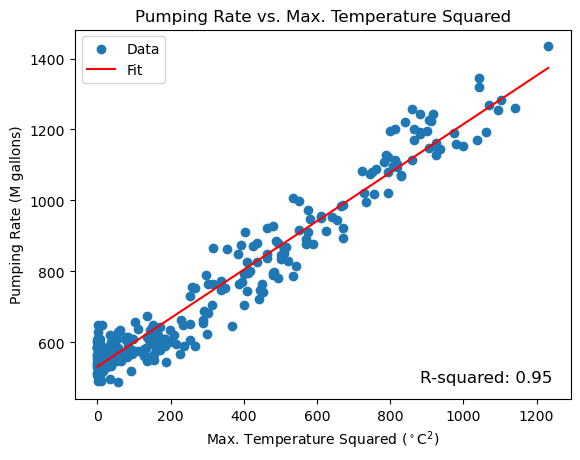
\includegraphics{report_files/figure-pdf/fig-temp-scatter-output-1.png}

}

\caption{\label{fig-temp-scatter}Scatter plot with model fit of pumping
rates vs.~maximum temperature squared. The model suggests that
temperature alone explains almost 95\% of the variability in pumping
rates (\(R^2 = 0.948\)).}

\end{figure}%

Given that there is high probability that temperature will continue to
increase in the future due to climate change, the results from our
analysis suggest that pumping rates will also increase in the future in
order to meet this growing atmospheric demand. In addition, if
population continues to grow, as expected, this will create additional
demand on our groundwater resources.

It is important to note that these results are based on the past 23
years of data. As population continues to grow and interventions, such
as fixing leaky pipes, take place, these relationships may change. In
order to more accurately predict future scenarios, a more complex
analysis, using a physics- or statistically-based model, is recommended.

\subsection{Conclusion}\label{conclusion}

We define sustainable aquifer conditions as those in which groundwater
depth is either not changing or increasing over time. Over the past 23
years the Missoula Aquifer has been incredibly resilient and even with
varying pumping rates, all groundwater wells show an overall increasing
water table elevation. However, over the most recent 10-years of data,
all groundwater levels are decreasing and most of them significantly.
This is likely due to the smaller increasing trend in recharge from the
river and increasing pumping rates from the City. Additionally, when the
trend in the river is removed from the groundwater time series, overall
trends in the water table depth are reduced and trends in shorter time
periods follow, inversely, the trends in pumping rates. These trends in
pumping rates are strongly driven by temperature and, more subtely,
driven by population. We believe that if temperature and population
continue to grow, that pumping rates will increase to match demand, thus
creating an unsustainable aquifer condition if recharge rates from the
river stabilize, or worse decrease. Given these results, we believe
that, while the groundwater table has been historically stable over the
period of record, the City should not rest on these laurels and should
continue to look for ways to mitigate the impacts of increasing
population and climate change in the valley.

\subsection{References}\label{references}

\phantomsection\label{refs}
\begin{CSLReferences}{1}{0}
\bibitem[\citeproctext]{ref-clevelandSTLSeasonaltrendDecomposition1990}
Cleveland, Robert B., William S. Cleveland, Jean E. McRae, and Irma
Terpenning. 1990. {``{STL}: {A} Seasonal-Trend Decomposition.''}
\emph{J. Off. Stat} 6 (1): 3--73.

\bibitem[\citeproctext]{ref-kendallRankCorrelationMethods1975}
Kendall, Maurice George. 1975. {``Rank Correlation Methods.''}

\bibitem[\citeproctext]{ref-lambrechtMeteostatPython2024}
Lambrecht, Christian Sebastian. 2024. {``Meteostat {Python}.''}

\bibitem[\citeproctext]{ref-mannNonparametricTestsTrend1945}
Mann, Henry B. 1945. {``Nonparametric Tests Against Trend.''}
\emph{Econometrica: Journal of the Econometric Society}, 245--59.
\url{https://www.jstor.org/stable/1907187}.

\bibitem[\citeproctext]{ref-millerNumericalFlowModel1991}
Miller, Ross. 1991. {``Numerical Flow Model of the {Missoula Aquifer} :
Interpretation of Aquifer Properties and River Interaction.''}
\emph{Graduate Student Theses, Dissertations, \& Professional Papers},
January.

\bibitem[\citeproctext]{ref-montanadnrcMontanaDroughtManagement2023}
Montana DNRC. 2023. {``Montana {Drought Management Plan}.''} Helena, MT.

\bibitem[\citeproctext]{ref-tallmanSourcesWaterCaptured2005}
Tallman, Amelia. 2005. {``Sources of Water Captured by Municipal Supply
Wells in a Highly Conductive Aquifer Western {Montana}.''}
\emph{Graduate Student Theses, Dissertations, \& Professional Papers},
January.

\bibitem[\citeproctext]{ref-whitlock2017MontanaClimate2017}
Whitlock, Cathy, Wyatt F Cross, Bruce D Maxwell, Nick Silverman, and
Alisa A Wade. 2017. {``2017 {Montana Climate Assessment}: {Stakeholder}
Driven, Science Informed,''} September, 1--269.
\url{https://doi.org/10.15788/M2WW8W}.

\end{CSLReferences}



\end{document}
